\section{Kubernetes. Pods communication. Service. Multiple Pods. Headless Service. Pod replicas.}

Общение с подами может проходит через http (через nginx).

Сервис балансирует запросы между подами.

\begin{figure}[H]
	\centering
	\begin{minipage}[b]{0.4\textwidth}
		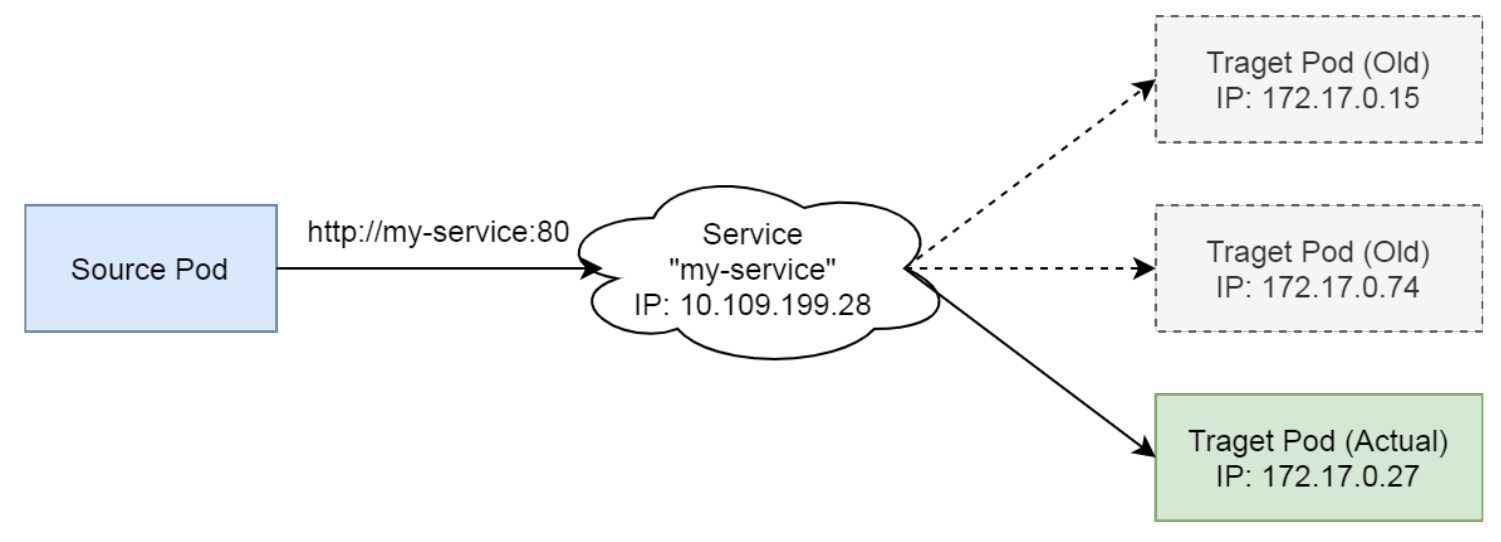
\includegraphics[width=\textwidth]{images/ssch.png}
        \caption{Service scheme}
	\end{minipage}
    \begin{minipage}[b]{0.4\textwidth}
		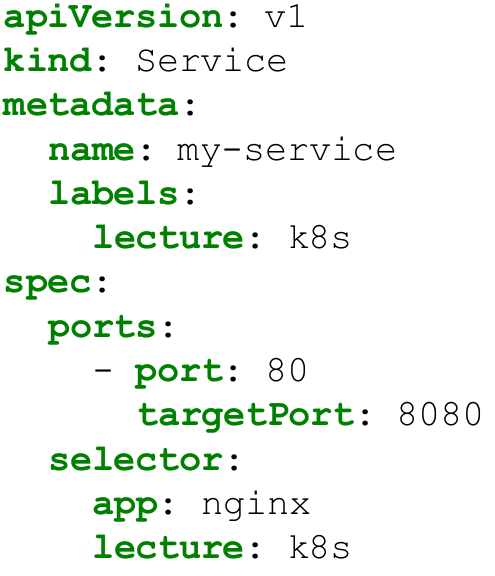
\includegraphics[width=\textwidth]{images/scon.png}
        \caption{Service config}
	\end{minipage}
\end{figure}

\begin{figure}[H]
	\centering
	\begin{minipage}[b]{0.4\textwidth}
		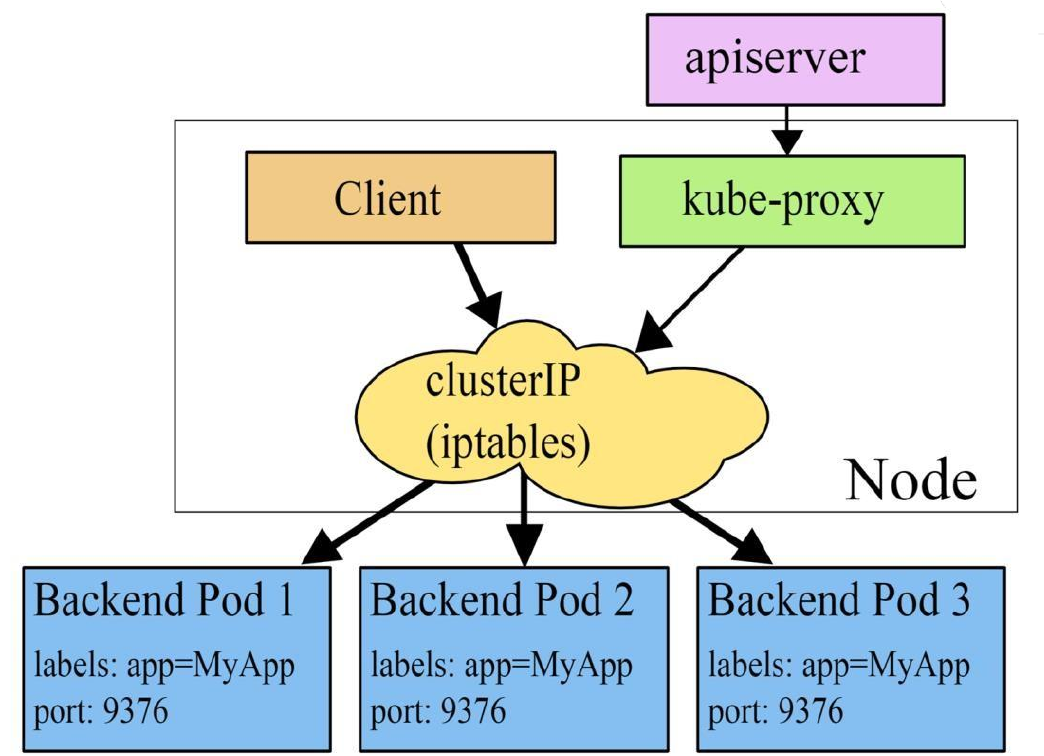
\includegraphics[width=\textwidth]{images/kapp.png}
        \caption{App scheme scheme}
	\end{minipage}
\end{figure}

Сервис - не пингуемый объект.

\subsection*{Multiple Pods}

В сервисе прописаны IPшники nginxов, на которых реализованы поды.

Запросы к подам подаются изолировано и поды друг о друге не знают.

Headless sercice - сервис без айпишника -> к нему нельзя обратиться напрямую.
\begin{figure}[H]
	\centering
	\begin{minipage}[b]{0.4\textwidth}
		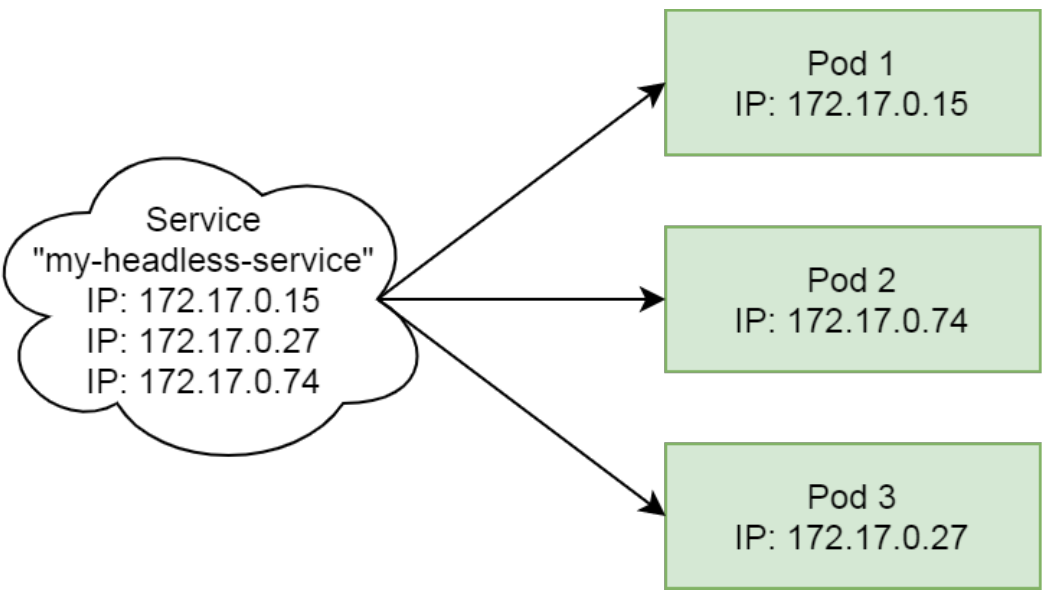
\includegraphics[width=\textwidth]{images/hls.png}
        \caption{Headless service}
	\end{minipage}
\end{figure}

\subsection*{Pod replicas}

Минусы отдельных серверов по конфигам:
\begin{itemize}
    \item Не масштабируются
    \item сложно поддерживать
    \item низкая оперативность
\end{itemize}
